\documentclass{beamer}

\usepackage[spanish]{babel}
\usepackage{listings}
\selectlanguage{spanish}
\usepackage[utf8]{inputenc}
\setbeamersize{text margin left=10mm,text margin right=3mm}

\title % (optional, only for long titles)
{TypeScript}
\author[Author, Anders] % (optional, for multiple authors)
{Sergio Álvarez Alonso \\ Adrián Mínguez Graña \\  Mario Moraño Orviz \\ 
Ángel Manuel Méndez Campal}
\institute[Universities Here and There] % (optional)
{
	\inst{}%
	Máster ingeniería web\\
	Universidad de Oviedo

}
\date[KPT 2004] % (optional)
{Diciembre 2018}
\subject{Computer Science}

\lstdefinestyle{customc}{
	belowcaptionskip=1\baselineskip,
	breaklines=true,
	frame=L,
	xleftmargin=\parindent,
	language=C,
	showstringspaces=false,
	basicstyle=\footnotesize\ttfamily,
	keywordstyle=\bfseries\color{green!40!black},
	commentstyle=\itshape\color{purple!40!black},
	identifierstyle=\color{blue},
	stringstyle=\color{orange},
}

\begin{document}
	
	\frame{\titlepage}
	
\small
\begin{frame}{Contexto y motivación del lenguaje I}
\begin{columns}[T] % contents are top vertically aligned
	\begin{column}[T]{8cm} % each column can also be its own environment

		\begin{itemize}
			\item Lanzado primera vez en 2012 (versión 0.8)
			\item 2 años de desarrollo interno en Microsoft
			\item Limitaciones de js para desarrollos de gran escala
			\item ``Adelanto'' de lo que cabría esperar de ECMAScript2015
			\item Anders Hejlsberg (LA de C\#) involucrado en el desarrollo
			\item Se transcompila a javascript
			\item Licencia Apache 2 (open source)
			\item Versión estable 3.1.6, 1 Noviembre
		\end{itemize}
	
	\end{column}
	\begin{column}[T]{3cm} % alternative top-align that's better for graphics
		
\includegraphics[height=3cm]{imagenes/ts.png}
		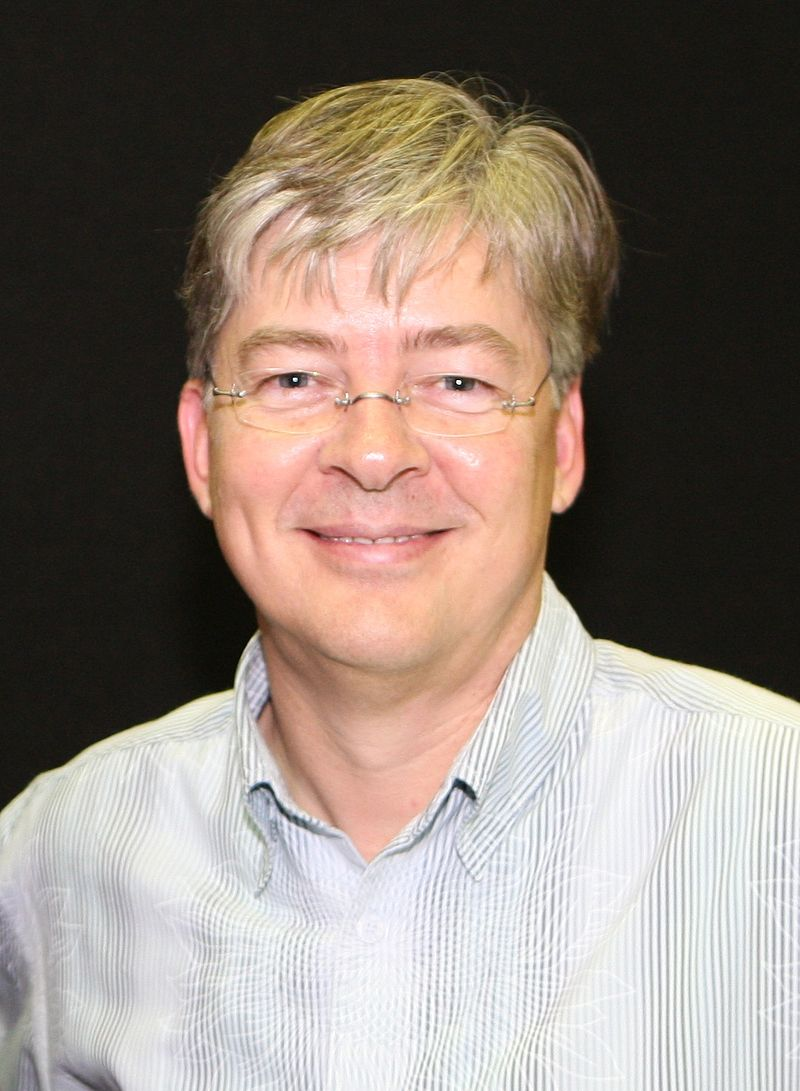
\includegraphics[height=3cm]{imagenes/anders.jpg}
	\end{column}

\end{columns}

\begin{block}{Herramientas}
	Al principio sólo Visual Studio. Luego Eclipse, Emacs, Vim, Sublime, Webstorm,
	Atom y Visual Studio Code.
\end{block}

\end{frame}


\begin{frame}{Contexto y motivación del lenguaje II}
\begin{columns}[T] % contents are top vertically aligned
	\begin{column}[T]{7cm} % each column can also be its own environment
		Objetivos:
		\begin{itemize}
			\item Dotar js con un sistema opcional de tipos
			\item Proveer a los motores de js actuales de características planeadas para versiones futuras
		\end{itemize}
		Superset de javascript: .js $\to$ .ts y compilar devuelve js válido \\
		
		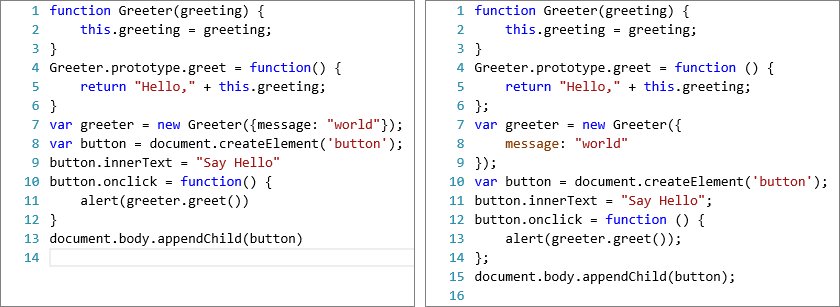
\includegraphics[height=3cm]{imagenes/ts3.png}
	
		
	\end{column}
	\begin{column}[T]{3cm} % alternative top-align that's better for graphics
		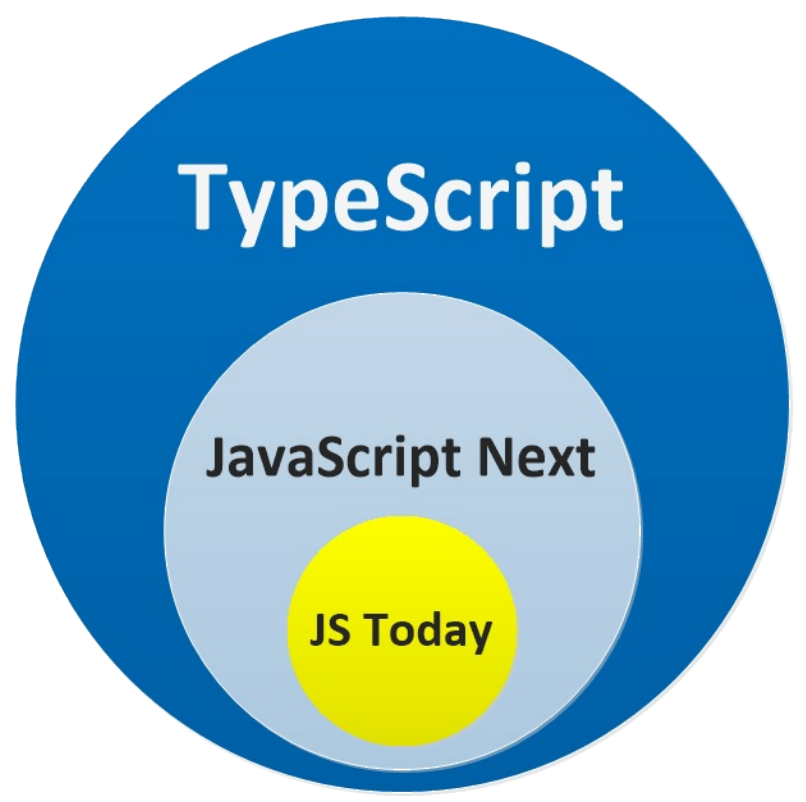
\includegraphics[height=3cm]{imagenes/ts2.png}
		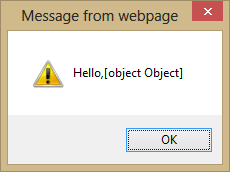
\includegraphics[height=3cm]{imagenes/ts4.png}
	\end{column}
\end{columns}

\end{frame}

\small
\begin{frame}{Contexto y motivación del lenguaje III}
\begin{columns}[t, onlytextwidth]
	\begin{column}[T]{.6\textwidth} % each column can also be its own environment
		
		Añade anotación de tipos que se borra al transcopilar\\
		Más información en tiempo de compilación \\
		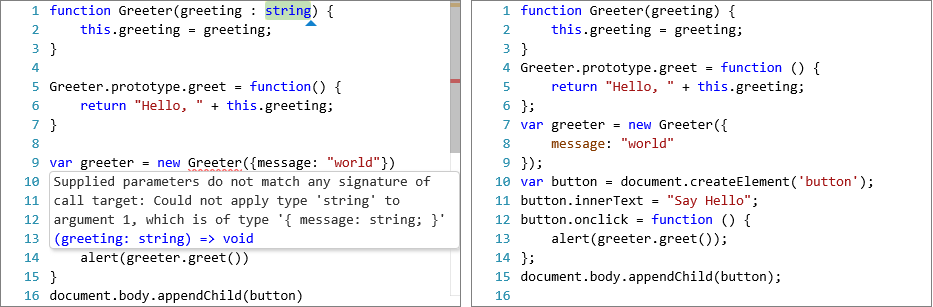
\includegraphics[height=2.5cm]{imagenes/ts5.png}
		
		Declaración de clases y modularidad \\
		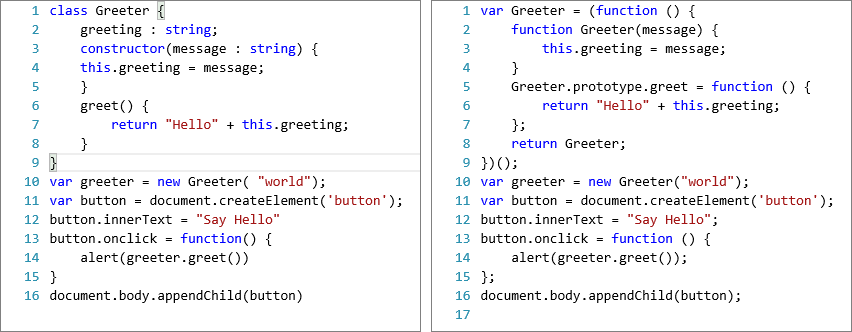
\includegraphics[height=2.5cm]{imagenes/ts7.png}
		
		
	\end{column}
	\begin{column}[T]{0.3\textwidth} % alternative top-align that's better for graphics
		IntelliSense
		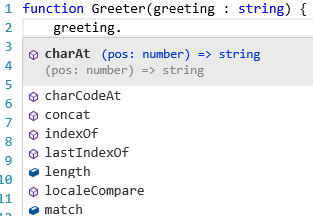
\includegraphics[height=2cm]{imagenes/ts6.png} \\ 
		\hfill \break
		\\
		
		Sintaxis de declaración de tipos de ECS6 \\
		Produce código js preparado para hacer
		herencia por prototipos \\
		
		
\includegraphics[height=2cm]{imagenes/ts8.png}
	
	\end{column}
\end{columns}
Escalar sitios web a aplicaciones más grandes

\end{frame}


\begin{frame}[fragile]
\frametitle{Principales características I}

\small
\begin{columns}[T]
	\begin{column}[T]{.5\textwidth} % each column can also be its own environment
		
		\begin{itemize}
			\item Orientación a objetos
			\item Transcompilación a js 
			\item Fuertemente tipado (estático) y comprobación de tipos en tiempo de ejecución
			\item Primitivos: number, boolean, string
			\item Tipo any (tipado débil, dinámico) similar EC6
		\end{itemize}
		
		
	\end{column}
	\begin{column}[T]{0.5\textwidth} % alternative top-align that's better for graphics
		\begin{itemize}
			\item npm gestor de dependencias
			\item cross platform
			\item TSC: compilador escrito en ts
			\item Tipos enum, void. Inferencia de tipos
		\end{itemize}

	\end{column}
\end{columns}

\tiny
 \begin{lstlisting}[style=customc, frame=single]
/** Funcion con tipo de retorno number. */
funcion restar (n1: number, n2: number): 
	number {return n1 - n2;}
	
/** Funcion sin tipo de retorno. Se infiere de los parametros y el return */
funcion restar () (n1: number, n2:number)
	{return n1 - n2;}
\end{lstlisting}


\end{frame}


\begin{frame}[fragile]
\frametitle{Principales características II}
Posibilidad de definir tus propios ''tipos'' a partir de otros tipos primitivos. 
\small
\begin{lstlisting}[style=customc, frame=single]
type Contador = number | string;

funcion mostrarAsignaturas (asignatura: Contador): string {
	return `Tengo ${asignatura} asignaturas.`;
}
\end{lstlisting}
Se define contador de tipo number o string. El parámetro de entrada de la función es de tipo contador
por lo que puede ser uno de ambos tipos primitivos. 

Soporta parámetros opcionales

\begin{lstlisting}[style=customc, frame=single]
function funcionConParametroOpcional(nombre: string, 
	age?: number)
\end{lstlisting}

\end{frame}

\begin{frame}[fragile]
\frametitle{Principales características III}
Interfaces. Siguiendo la filosofía de ser un lenguaje orientado a objetos y basado en clases.
Durante la transcompilación de código .ts a .js, las interfaces no generan código EC6. 
Simplemente se utilizan durante el desarrollo typescript a modo de ''contratos''.
\begin{lstlisting}[style=customc, frame=single]
interface Persona {
	nombre: string;
}

let a: Persona = {
	nombre: 'Pedro'
}
\end{lstlisting}
\end{frame}

\begin{frame}
\frametitle{Conclusiones}
	\begin{itemize}
		\item Buena curva de aprendizaje 
		\item Es necesario saber javascript (misma sintaxis y semántica)
		\item Permite reusar js y sus librerías
		\item Produce código limpio y garantiza compatibilidad con el navegador
		\item Escalabilidad
		\item Open source
		\item Comunidad activa
		\item Menos código que en js. Ahorra tiempo
		\item Código más legible
		\item En pleno desarrollo
		
	\end{itemize}
\end{frame}


\begin{frame}{Referencias}
\begin{itemize}  
	\item https://blogs.msdn.microsoft.com/somasegar/2012/10/01 \\ /typescript-javascript-development-at-application-scale/
	\item TypeScript Deep Dive. Basarat Ali Syed. 
	\item https://fullstack-developer.academy/debugging-typescript-in-the-browser/
	\item https://www.typescriptlang.org/
	\item https://dzone.com/articles/what-is-typescript-and-why-use-it
\end{itemize}
\end{frame}


\end{document}